\documentclass[14pt,a4paper]{extarticle}
\usepackage{graphicx}
\usepackage[T1]{fontenc}
\usepackage[utf8x]{inputenc}
\usepackage{pdfpages}
\usepackage{libertine}
\usepackage{amsmath}
\usepackage{amssymb}
\usepackage{listings}
\usepackage{color} %red, green, blue, yellow, cyan, magenta, black, white
\usepackage{float}
\usepackage{hyperref}

\begin{document}
	\begin{titlepage}
		\centering
		{\scshape\LARGE Swapindo \par}
		\vspace{2.5cm}
		{\huge\bfseries Installationsbeschreibung Mutual Authentication \par}
		\vfill
		von\par
		Benjamin Ellmer (\textsc{S1910237013})
	
		\vfill
		{\large \today\par}
	\end{titlepage}
	\newpage

	\tableofcontents
	\newpage
	
	\section{Vorwort}
	Das Ergebnis meines Projekts ist eine Library für die Mutual Authentication geworden.
	In diesem Dokument finden Sie eine Beschreibung, wie diese Library verwendet werden kann.
	In der Abgabe unter Implementierung finden Sie 4 Ordner: KeyManagment, JWT, mTLS und MutualAuthenticationLibrary.
	KeyManagment enthält alle files für das key management und eine Beispiel CA mit Beispiel keys. 
	Das Passwort für alle files ist B3njam1n.
	Unter JWT und mTLS finden Sie Beispielprojekte, die die Authentifizierungsmechanismen implementieren.

	\section{Installation}
	\noindent Library zu Projektmappe hinzufügen: \\
		Projektmappe -> Hinzufügen -> Vorhandenes Projekt 
	\vspace{1cm}

	\noindent Library zu Projektmappe hinzufügen: \\
		Abhängigkeiten -> Projektverweis hinzufügen -> MutualAuthenticationLibrary

	\section{Key Management}
	\noindent Keys für die CA erstellen, mittels: \\
	./create-ca.sh \textit{\$password} \textit{\$subject}
	\vspace{1cm}

	\noindent Keys für einen Service erstellen, mittels: \\
	./gen-service-keys.sh \textit{\$passwordService} \textit{\$passwordCA} \textit{\$subject} \textit{\$caPath}
	\vspace{1cm}

	\noindent Die pfx files der services müssen dann in die Projektverzeichnisse der services kopiert werden.
	Das ca.crt file muss auch in das Projektverzeichnisse aller services kopiert werden.

	\newpage

	\section{Implementierung mTLS}
	\subsection{Server}
	\subsubsection*{Zertifikatauthentifizierung erlauben (Program.cs)}
	\begin{center}
		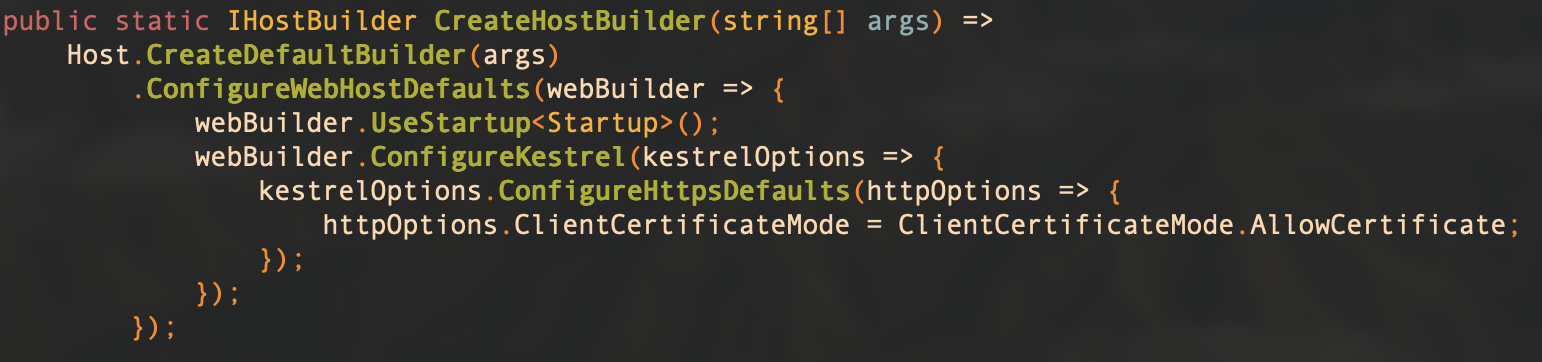
\includegraphics[width=\textwidth]{images/AllowCerts.png}
	\end{center}

	\subsubsection*{Certificate Authority Service hinzufügen (Startup.cs)}
	\begin{center}
		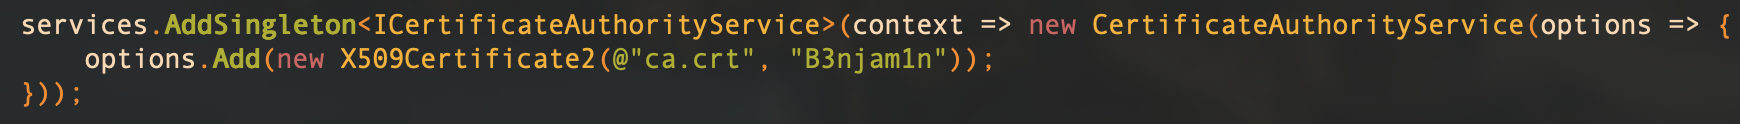
\includegraphics[width=\textwidth]{images/CAService.png}
	\end{center}

	\subsubsection*{MTLS Konfigurieren (Startup.cs)}
	\begin{center}
		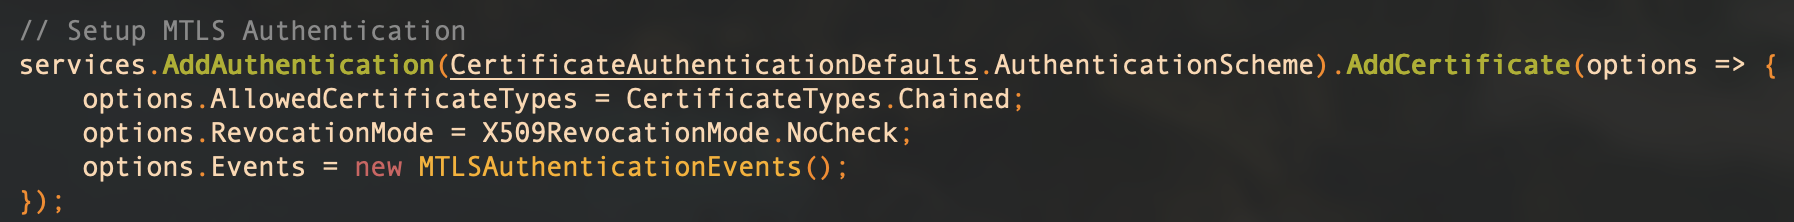
\includegraphics[width=\textwidth]{images/ConfigMTLS.png}
	\end{center}

	\subsubsection*{MTLS verwenden (Startup.cs)}
	\begin{center}
		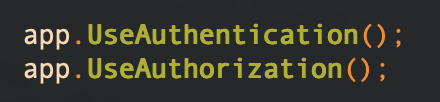
\includegraphics{images/UseMTLS.png}
	\end{center}
	\newpage

	\subsection{Client}
	\subsubsection*{MTLS Client hinzufügen (Startup.cs)}
	\begin{center}
		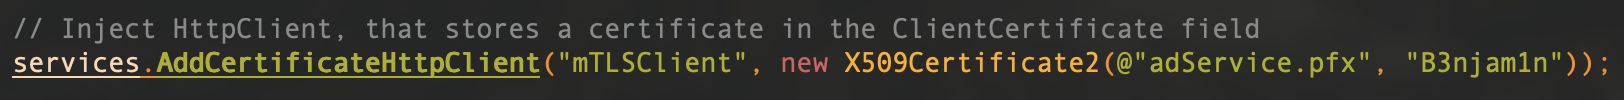
\includegraphics[width=\textwidth]{images/AddMTLSClient.png}
	\end{center}

	\subsubsection*{MTLS Client injecten (...Controller.cs)}
	\begin{center}
		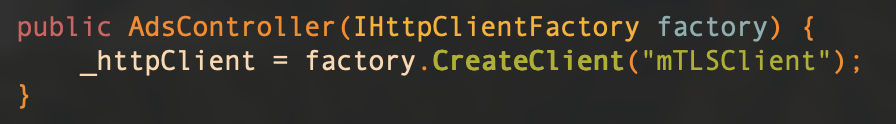
\includegraphics[width=\textwidth]{images/InjectClient.png}
	\end{center}


	\newpage
	\section{Implementierung self-signed JWT}
	\subsection{Server}
	\subsubsection*{Zertifikatauthentifizierung erlauben (Program.cs)}
	\begin{center}
		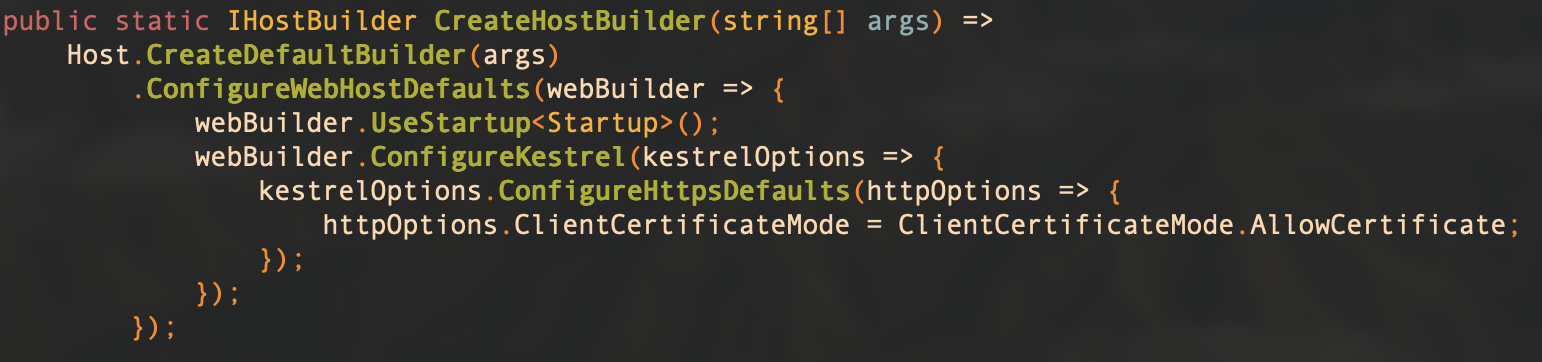
\includegraphics[width=\textwidth]{images/AllowCerts.png}
	\end{center}

	\subsubsection*{Certificate Authority Service hinzufügen (Startup.cs)}
	\begin{center}
		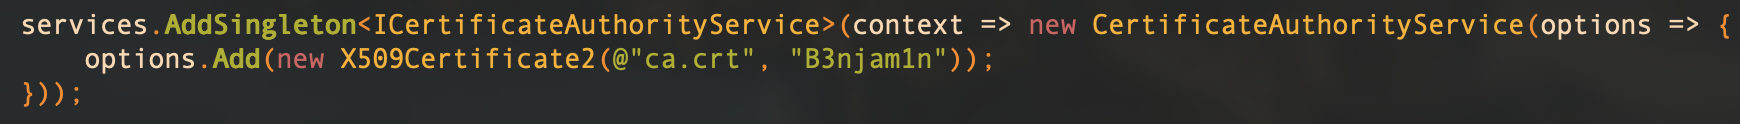
\includegraphics[width=\textwidth]{images/CAService.png}
	\end{center}
	
	\subsubsection*{Token Validation Service hinzufügen (Startup.cs)}
	\begin{center}
		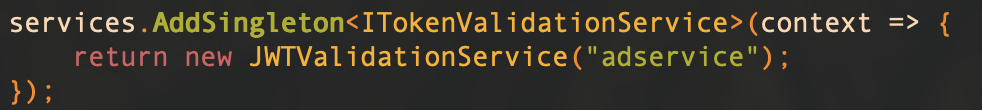
\includegraphics[width=\textwidth]{images/AddTokenValidator.png}
	\end{center}

	\subsubsection*{Token Authentifizierung aktivieren (Startup.cs)}
	\begin{center}
		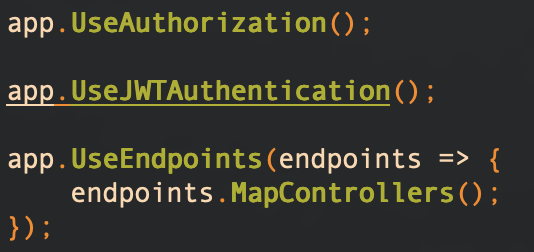
\includegraphics{images/UseAuth.png}
	\end{center}

	\newpage
	\subsection{Client}

	\subsubsection*{Token Creator Service hinzufügen (Startup.cs)}
	\begin{center}
		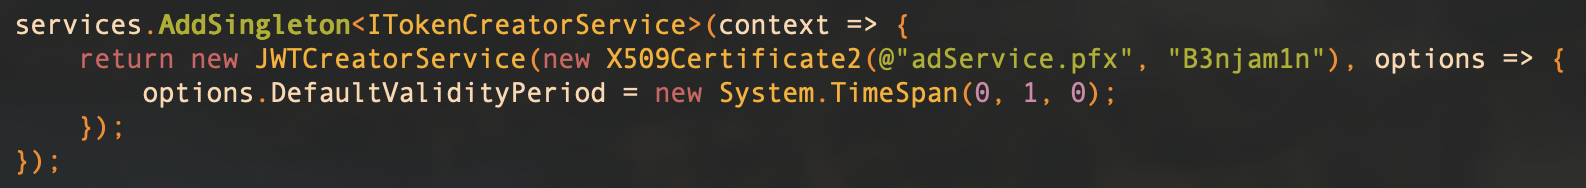
\includegraphics[width=\textwidth]{images/AddTokenCreator.png}
	\end{center}
	
	\subsubsection*{Http Clients hinzufügen (Startup.cs)}
	\begin{center}
		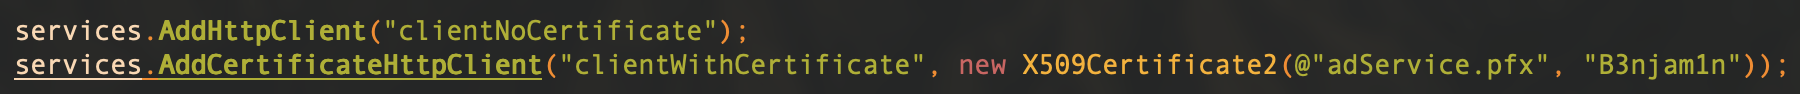
\includegraphics[width=\textwidth]{images/AddHttpClients.png}
	\end{center}

	\subsubsection*{Http Clients Injecten (...Controller.cs)}
	\begin{center}
		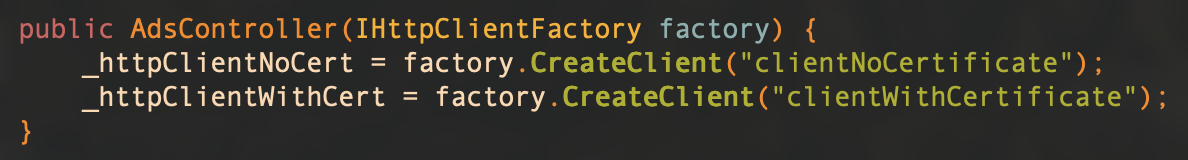
\includegraphics[width=\textwidth]{images/InjectClients.png}
	\end{center}

\end{document}

